\subsection{Induction on Proof Trees}
\label{sec:induction-on-proof-trees}
This type of induction is used to prove that a statement exhibits given behaviour.
Since often, we are not restricted to just simple statements, such where we know that we are applying the $\textsc{Ass}_{\text{NS}}$ rule,
we need to perform case distinction on all possible last rules applied in the derivation tree $T$.
If all are to be proven, this will yield $7$, one for each rule of the big-step semantics.

\inlinedefinition[Subderivation] We define $T' \sqsubset T$, where $T$ is a derivation tree. $T'$ is called a \textit{subderivation} of $T$,
or more simply, a \textit{subtree} of $T$. Definition is analogous to the subterm relation.


\shade{ForestGreen}{Rundown} Below a rundown of how such proofs are expected to be laid out.

We define $P(T) \equiv \forall \sigma, \sigma', s . (\texttt{root}(T) \equiv \text{statement})$.
The quantifier-bound variables / states / statements can of course differ, so adjust accordingly.
This step is the crucial step to setting up this type of induction.

We then prove $\forall T . P(T)$ by strong induction on the shape of the derivation tree $T$.
Thus, for some arbitrary $T$, the induction hypothesis is $\forall T' \sqsubset T . P(T')$ and we prove $P(T)$.

Let $\sigma, \sigma', s$ (and more, if applicable) be arbitrary.

Then, for rules, such as $\textsc{WhT}_{\text{NS}}$, we draw up a derivation tree, like so (from solutions of Exercise Session 11, FS2026):
\begin{center}
    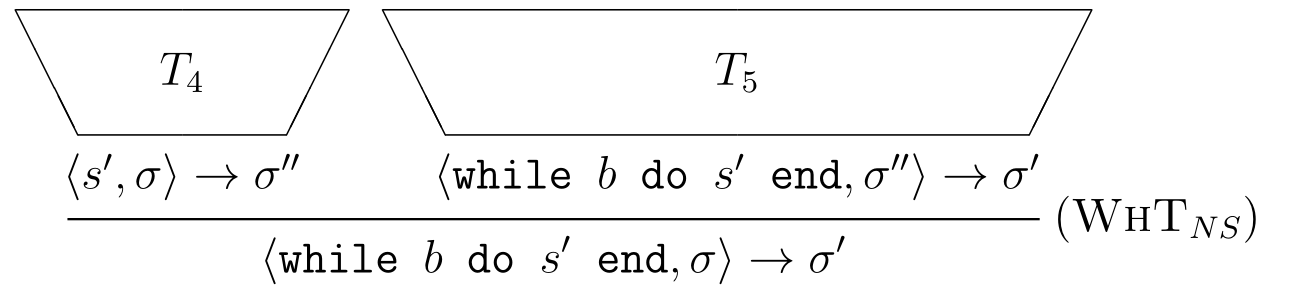
\includegraphics[width=0.6\linewidth]{assets/proof-on-shape-of-tree.png}
\end{center}
After it, we need to put final constraints and bind free variables in some way, e.g. here:

For some $b, s', \sigma'', T_4, T_5$, such that $s \equiv \texttt{while}\; b \; \texttt{do} \; s' \; \texttt{end}$ and $\cB \llbracket b \rrbracket \sigma = \texttt{tt}$.

Then use the induction hypothesis on the subderivations $T_i$ and finish the proof by showing the original statement holds under the induction hypothesis.
